\section{02.10.2024}{Grafy Cayleya}

\subsection{Metryka słów}

\begin{definition}{metryka słów}{}
  Niech $G$ będzie grupą, a $S$ dowolnym układem jej generatorów. Wówczas dla dowolnych $g_1,g_2\in G$ \buff{odległość między nimi w metryce słów} definiujemy jako
$$ds(g_1, g_2)=\min\{n\;:\;g_2=g_1s_1,...,s_n,\;s_i\in S\cup S^{-1}\},$$
gdzie $S^{-1}=\{g^{-1}\;:\;g\in S\}$.
\end{definition}

Metryka słów jest 
\begin{enumerate}
  \item skończona
  \item symetryczna (z definicji generatorów)
  \item \hl{lewo-niezmiennicza}, czyli $(\forall\;\gamma\in G)\;ds(\gamma g_1,\gamma g_2)=ds(g_1, g_2)$
\end{enumerate}
Ostatnia własność oznacza, że $G$ działa na sobie jako na przestrzeni metrycznej przez izometrie.

Gromov chce patrzeć na dyskretne przestrzenie metryczne, jakimi są grupy z metryką słów, jako na przestrzenie ciągłe (z dużej odległości).

\subsection{Graf Cayleya}

\begin{definition}{graf Cayleya}{}
Niech $G$ będzie grupą, a $S$ zbiorem jej generatorów. $C(G, S)$ to graf Cayleya o wierzchołkach będących elementami $G$ i skierowanych krawędziach etykietowanych generatorami:
\begin{center}
  \begin{tikzcd}
    g\arrow["s", r] & gs
  \end{tikzcd}
\end{center}
gdzie $g\in G$ i $s\in S$.
\end{definition}

\begin{example}[m]
\item Dla $G=\Z^2$ oraz $S=\{{\color{red}\overbrace{(1, 0)}^s}, {\color{blue}\overbrace{(0, 1)}^t}\}$ graf Cayleya to nieskończona "kratka"
  \bigskip

  \begin{center}
    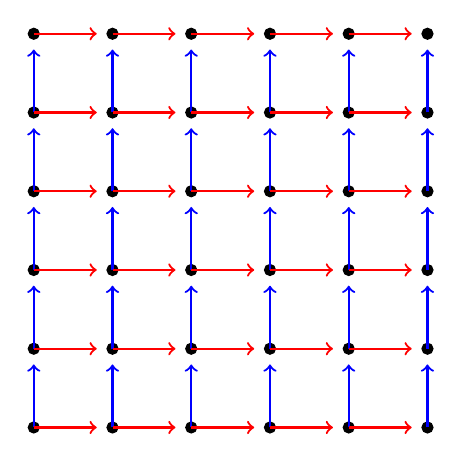
\begin{tikzpicture}
      \foreach \x in{0,...,5} { 
        \foreach \y in{0,...,5} {
          \filldraw (\x, \y) circle (2pt);
        }
      }

      \foreach \x in {0,...,5} {
        \foreach \y in {0,..., 4} {
          \draw[->, blue, thick] (\x, \y) -- (\x, \y+.8);
        }
      }
      \foreach \x in {0,...,4} {
        \foreach \y in {0,..., 5} {
          \draw[->, red, thick] (\x, \y) -- (\x+.8, \y);
        }
      }
    \end{tikzpicture}
  \end{center}
\item Dla grupy cyklicznej rzędu $p$ z generatorem $\color{red}s$ graf Cayleya to $p$-kąt
  \begin{center}
    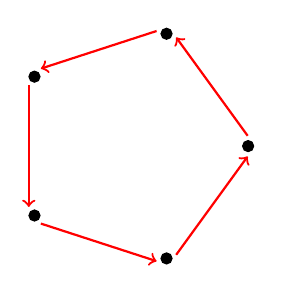
\begin{tikzpicture}
      \foreach \i in {0,..., 4} {
        \filldraw ( 360 /5 * \i :1.5) circle (2pt);
        \draw[->, red, thick] (360/5*\i + 5:1.5) -- (360/5*\i + 360/5 - 5:1.5);
      }
    \end{tikzpicture}
  \end{center}
\item {\color{red}\Large TO DO} parkietarz kwadratami
\end{example}

Każdy graf Cayleya jest \buff{spójny}, bo jego krawędzie to mnożenie przez generatory. Dodatkowo, grupa $G$ działa na nim przez \hl{automorfizmy zachowując krawędzie oraz ich etykiety}. To znaczy, że krawędż z wierzchołkami \begin{tikzcd}g\arrow[r, "s"]&gs\end{tikzcd} pod działaniem elementu $\gamma \in G$ staje się \begin{tikzcd}\gamma g\arrow[r, "s"] & \gamma gs\end{tikzcd}.

Jeśli każdą krawędź w grafie Cayleya potraktujemy jako odcinek długości $1$, to możemy na nim zdefiniować metrykę która jako odległość dwóch punktów przyjmuje długość najkrótszej ścieżki między nimi. Ta metryka na wierzchołkach pokrywa się z \buff{metryką słów} na grupie $G$ o generatorach $S$, której graf rozpatrujemy. Przy takiej metryce działanie grupy $G$ jest więc działaniem nie tylko przez automorfizmy, ale przez izometrie (lewa-niezmienniczość).

Innym wariantem grafu Cayleya jest graf w którym wierzchołki są elementami grupy $V=G$, ale krawędzie są niezorientowane: $E=\{\{g_1, g_2\}\;:\;ds(g_1,g_2)=1\}$. W przykładzie z parkietarzem zamiast podwójnych krawędzi w obie strony będzie on miał pojedyńczą, nieskierowaną krawędź


Dla surjekcji $\pi:F_S\to G$, gdzie $G=\langle S\;|\; R\rangle=F_S/N$ możemy mieć dwie tak samo zorientowane strzałki między dwoma wierzchołkami (gdy np. $g_1\pi(s_1)=g_1\pi(s_2)=g_2$
\begin{center}
  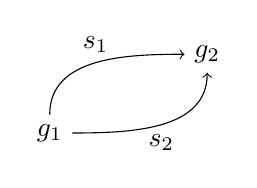
\begin{tikzpicture}
    \node (g1) at (0, 0) {$g_1$};
    \node (g2) at (2, 1) {$g_2$};
    \draw[->] (g1) to [out=90, in=180] node[midway, above] {$s_1$} (g2);
    \draw[->] (g1) to [out=0, in=-90] node[midway, below] {$s_2$} (g2);
  \end{tikzpicture}
\end{center}

Graf Cayleya grupy wolnej to nieskończone drzewo stopnia równego ilości $2\cdot$ ilość generatorów. 

\begin{definition}{suma drzewiasta}{}
  Mając dwie grupy $(G_1, S_1)$ i $(G_2, S_2)$ graf Cayleya ich sumy wolnej, czyli graf $(G_1\star G_2, S_1\cup S_2)$ to graf pierwszej grupy, który w każdym wierzchołku ma kopię grafu drugiej grupy, która w każdym wierzchołku ma kopię pierwszej grupy...

  \begin{center}
    \begin{tikzpicture}

    \end{tikzpicture}
  \end{center}
\end{definition}
